\documentclass{article}
\usepackage{graphicx}
\usepackage{multirow}
\usepackage{caption, subcaption}
\graphicspath{D:/Texmaker/grphics n tables/images/}

\begin{document}
\title {including graphics}

\section {Table Introduction}
\subsection{More on tables}
\begin{table}[htbp]
\caption{Text wrapping}
\begin{center}
%p tag wraps inside a cell
\begin{tabular}{| l | l | p{5 cm} |}
\hline
Programming & Texting\\
Languages &  Markup\\
Implementing & Deploy\\
\hline

\end{tabular}
\end{center}
\label{tab:wrapping}
\end{table}

\begin{table}[htbp]
\caption{Spanning Row and columns}
\begin{center}
%p tag wraps inside a cell
\begin{tabular}{| l | c | c |}
\hline
% & for black line 2 no of columns, centered, 
& \multicolumn{2}{c|}{Ranges}\\
& X & Y\\
\hline
% 3 rows * width of the column(natural)  text that will expand in three rows.
\multirow{3}{*}{Hot} & 7 & 9\\
&5 &6\\
&6 &7 \\
\multirow{3}{*}{cold} & 4 & 7\\
&5 &6\\
&5 &3 \\
\hline

\end{tabular}
\end{center}
\label{tab:multi}
\end{table}



\section{Introduction}
\begin{figure}
\centering
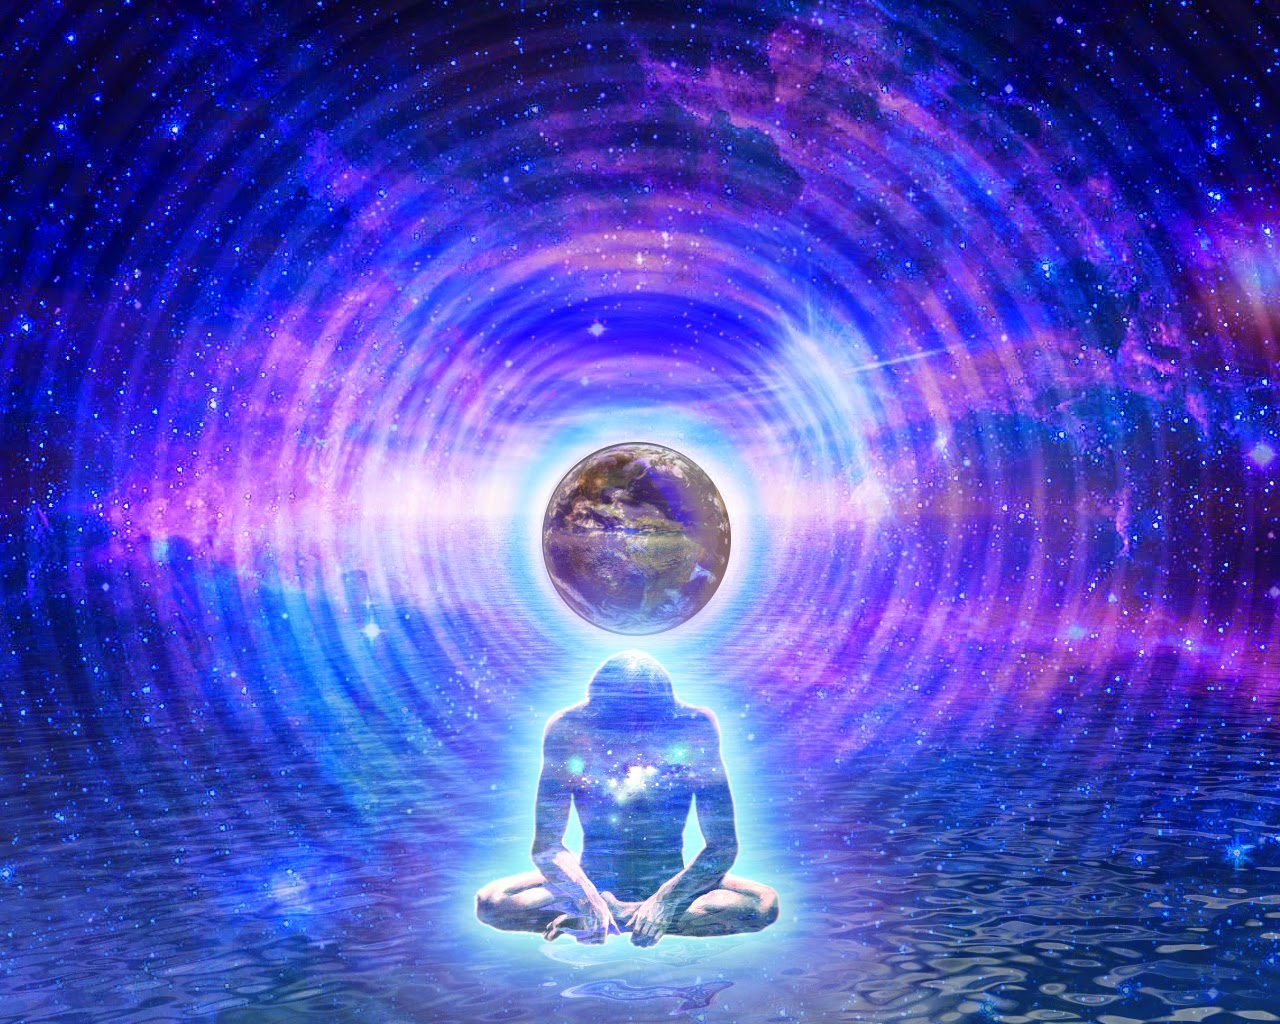
\includegraphics[width=0.7 in]{D:/Texmaker/grphics n tables/images/meditate.jpg}
\caption{Figure}
\label{meditate}
\end{figure}

\subsection{More on graphics}

\begin{figure}
\begin {center}

\begin{subfigure}[b]{0.2\textwidth}
\centering
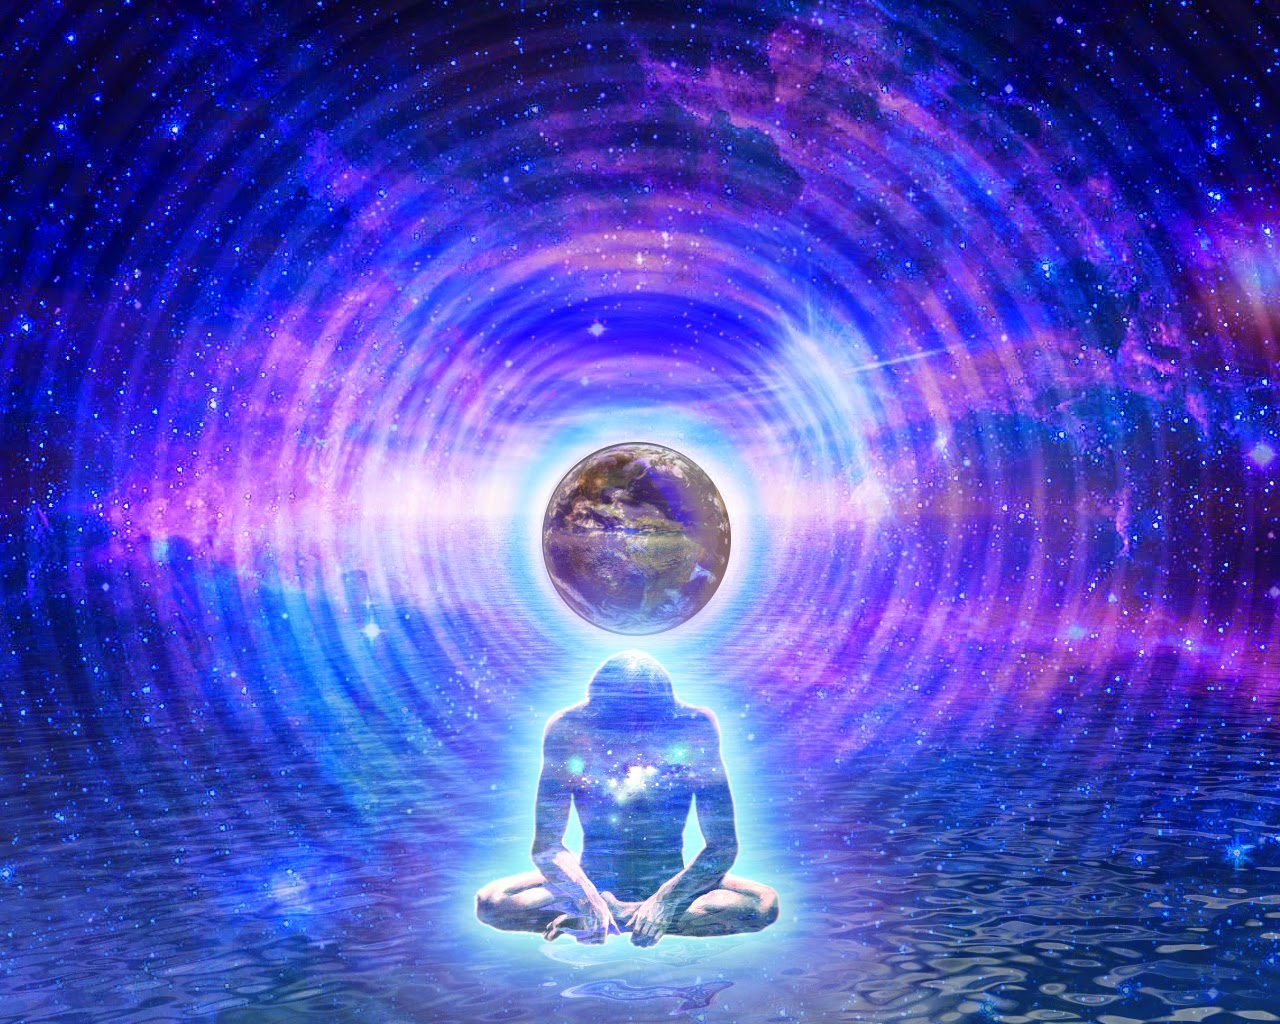
\includegraphics[width=0.5 in]{D:/Texmaker/grphics n tables/images/meditate.jpg}
\caption{Beginning}
\label{fig:meditate1}
\end{subfigure}

\begin{subfigure}[b]{0.2\textwidth}
\centering
% aligning two figures in line in two columns
%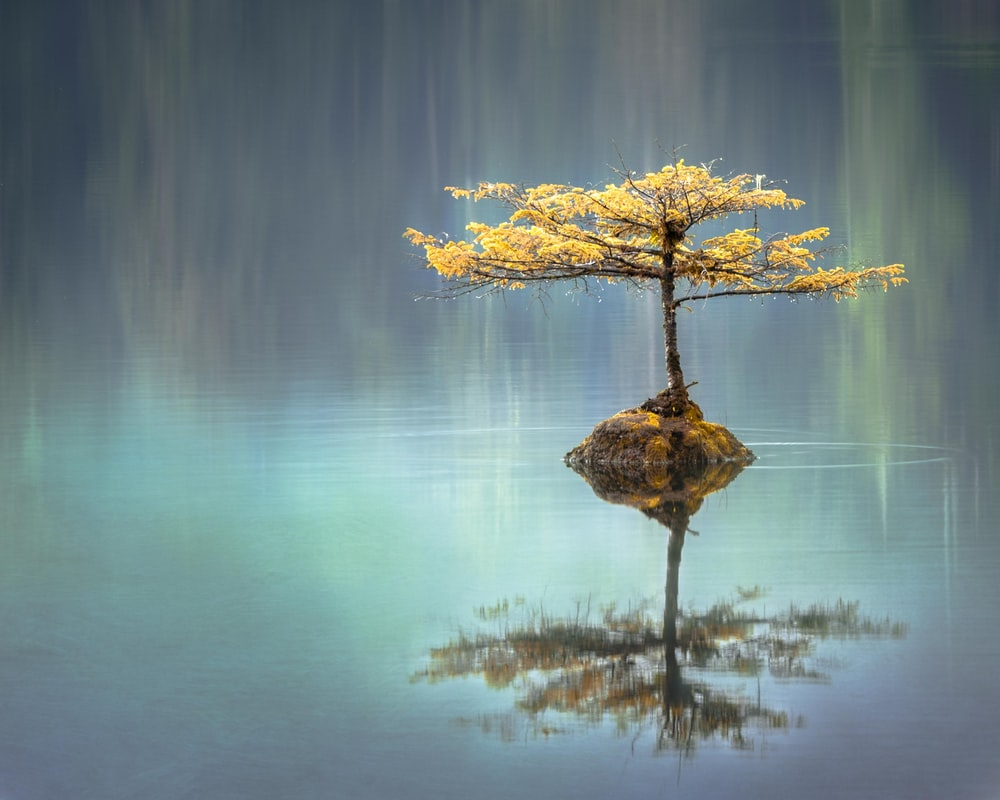
\includegraphics[scale=.5]{D:/Texmaker/grphics n tables/images/plant.jpg}
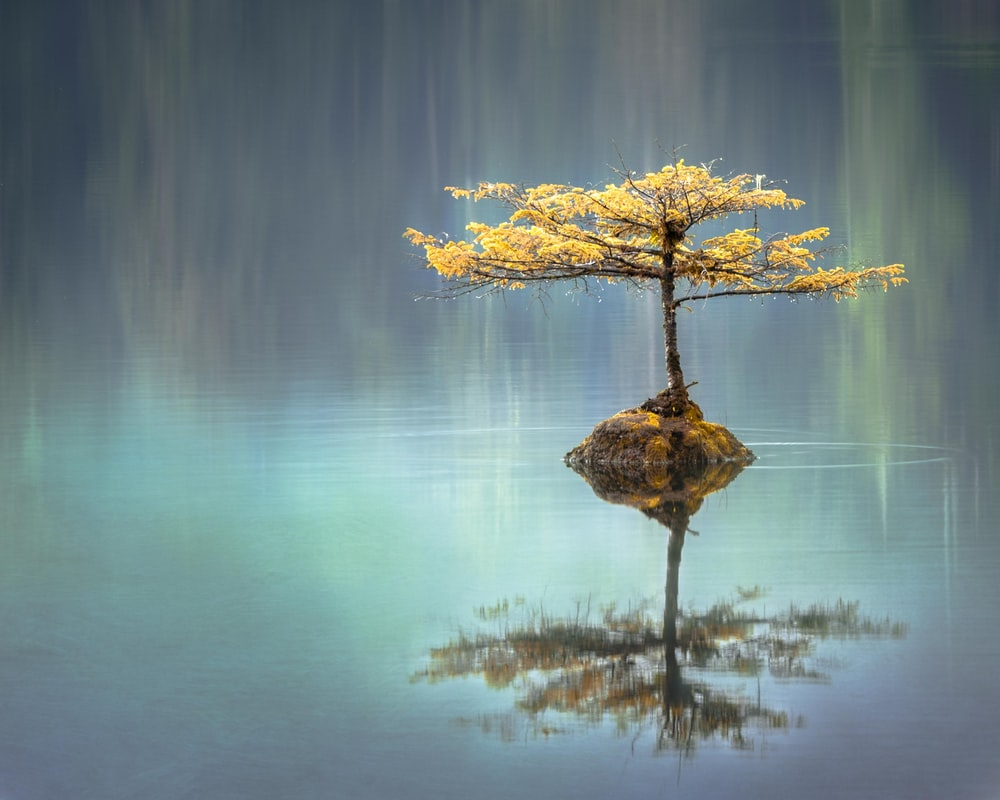
\includegraphics[width=0.5 in]{D:/Texmaker/grphics n tables/images/plant.jpg}
\caption{End}
\label{fig:plant1}
\end{subfigure}

\caption{Meditation}
\label{fig:subs}
\end {center}
\end{figure}






\subsection{Floating Figure Environment}
In my article , I am going to use jpg image in floating env. in Figure\ref{fig:plant}

\begin{figure}
% for centering env.
\begin{center}
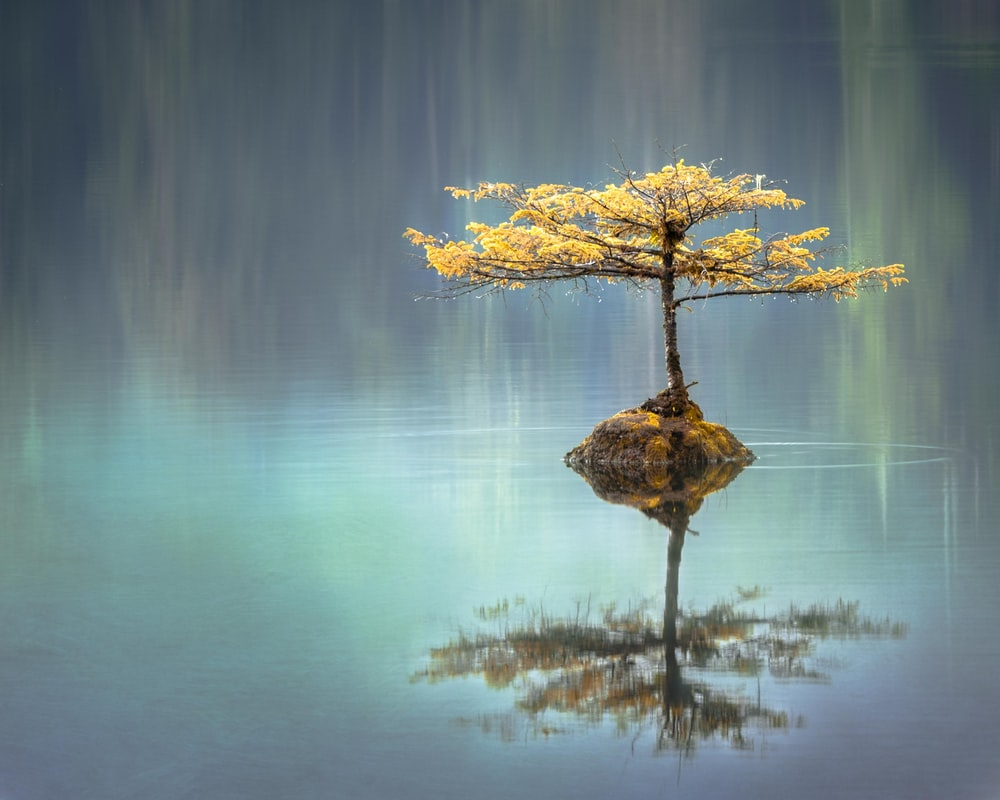
\includegraphics[width=0.7 in]{D:/Texmaker/grphics n tables/images/plant.jpg}
\caption{Plant}
\label{fig:plant}
\end{center}
\end{figure}

\end{document}